\documentclass[10pt,letterpaper]{ltugboat}
\usepackage{times,amsmath,graphicx,array,listings,ragged2e}
\usepackage[german,english]{babel}
\usepackage{verbatim}
%
\title{Using \MP { }to create a basic sewing pattern from individual measurements}
%
\author{%
{Dolores Messer{\small $~^{1}$}, Marium Zeeshan{\small $~^{1}$}, Prasenjit Saha{\small $~^{2}$}}%
% add some space between author names and affils
\vspace{1.6mm}\\
\fontsize{10}{10}\selectfont\itshape
$^{1}$\,$^{1}$\,$^{2}$\,Institute for Theoretical Physics, University of Zurich, Switzerland\\
\fontsize{9}{9}\selectfont\ttfamily\upshape
\\
$^{1}$\,dolores.messer@uzh.ch\\
$^{1}$\,marium.zeeshan@uzh.ch\\
$^{2}$\,psaha@physik.uzh.ch
% add some space between email and affil
\vspace{1.2mm}\\
\fontsize{10}{10}\selectfont\rmfamily\itshape
\footnote{\small $~^{1}$} Both are first author}

%%%%%%%

\begin{document}
\maketitle
%%%%%%%
\lstset{language=MetaPost}
%%%%%%%
\begin{abstract} 
\textit{Generate bodice sloper with \MP. General outcome: Can be done without problems if body shape is not special. Very sensitive to measurement errors. Challenge: dart creation, smooth transitions.}
\end{abstract}
%%%%%%%

%%%%%%%
\section{Introduction}
\par Sewing is one of the oldest textile arts, which is passed from generation to generation. For thousand of years, sewing has been done by hand using needles, whereas nowadays almost all sewing is done by sewing machines. Before a piece of clothing can be sewn together, the parts of the garment are traced onto fabric using a pattern and then cut out. The construction of the pattern is one of the more difficult tasks of the sewing process. Simple patterns are just based on specific measurements of the intended wearer, whereas more complex patterns involve a special design. There are basic patterns, called slopers, which are made to fit a particular individual exactly. From this basic pattern, other patterns can be drafted by pattern manipulation techniques. As the exact measurements vary from person to person, a sloper is different for each person. Since the basic construction of a sloper is done the same way for each individual, a lot of cumbersome work could be avoided by automating this process. Ideally, some kind of computer program is designed in order to automatically generate a customized sloper on the basis of specific individual measurements. This would not only reduce the work, but also decrease the complexity of the pattern creation process, since no prior knowledge of pattern making is required.
\par In this paper, we propose that the programming language \MP { }is well-suited to generate such a basic pattern. \MP { }is a versatile and simple language that supports graphics programming, and is particularly well-suited to generate figures, where the aspect of the figure may be controlled by mathematical or geometrical constraints that can be expressed symbolically. We wrote a program based on \MP, which creates the basic bodice sloper pattern for women suggested by Maddie Flanigan \cite{maddie} given some individual measurements. We chose to construct a sloper since we are not familiar with pattern design and the construction of a sloper does not involve any design. Anyone can use our program, it simply requires the user to take exact measurements. The main structure of our program is to generate the bodice sloper by using the individual measurements as input and creating a pdf-file as output.
\par \justifying Section 2 discusses some of the related programs provided by companies. In Section 3, the implementation of our \MP { }program and its challenges are discussed. Section 4 provides some conclusions with future directions that we plan to explore.
%%%%%%%

%%%%%%%
\section{Related programs}
There is a huge variety of commercial sewing pattern software on the market, with which custom-fitted patterns from both given and individual measurements can be drafted.\\
The most simple programs, such as \textit{Dress Shop} \cite{livingsoftnw}, \textit{My Pattern Designer} \cite{mypatterndesigner}, \textit{PASST!} \cite{golden}, \textit{Pattern Master} \cite{wildginger} and \textit{Schnittvision Couture Software} \cite{schnittvision}, do not require any prior knowledge of pattern making, and they usually come with a collection of patterns in standard sizes, that can be adjusted to individual measurements by changing some parameters. Additionally, they offer some design options such as variations in the collar style or sleeve design. The program CADTERNS \cite{cadterns} allows the user to create basic slopers from individual measurements. The skill of turning the slopers into patterns can be acquired in the affiliated Cyber School.\\
There is a multitude of much more complex computer-aided design (CAD) sewing pattern programs, which offer much more functionality, but require knowledge in manual pattern construction and are not that simple to handle.\footnote{Known programs are \textit{Akku Mark Pattern Design Software} \cite{gerber}, \textit{CAD Pattern Cutting Software} \cite{telestia}, \textit{Cameo} \cite{wildginger}, \textit{COAT} \cite{coat}, \textit{Designer v6i Software} \cite{designsew}, \textit{Digital Fashion Pro} \cite{digitalfashion}, \textit{Fashion CAD} \cite{fashioncad}, \textit{Fittingly Sew} \cite{fittinglysew}, \textit{Garment Designer} \cite{garmentdesigner}, \textit{Gemini Pattern Editor} \cite{gemini}, \textit{GRAFIS} \cite{grafis}, \textit{Lectra} \cite{lectra}, \textit{Marvelous Designer} \cite{marvelousdesigner}, \textit{Optitex} \cite{optitex}, \textit{PAD System} \cite{padsystem}, \textit{Pattern Maker} \cite{patternmaker}, \textit{STYLEtexpro CAD} \cite{styletexpro}, \textit{Tukatech} \cite{tukatech} and many more.} These programs are used in the fashion industry in order to design new patterns on the screen and offer a variety of functionalities such as the inclusion of measurements for the not so perfect body, manual or automatic pattern grading, simulation for darts, the use of existing slopers to create new styles of garment, 3D cloths simulation, office work etc.\\
In addition, there are some projects in order to create open source pattern making programs due to the fact that most current applications for pattern making are proprietary and expensive, and do not give much control on the creation process. Susan Spencer Conklin has been developing \textit{Tau Meta Tau Physica} \cite{taumeta}, a program written in Python that can be used to create design files by programming the design formulas. There is further a free java program called \textit{Pattern Designer} \cite{patterndesigner} which can be used in order to create slopers and patterns. \textit{SodaCAD} \cite{sodacad} is an open source pattern making CAD suite written in C++ and gtkmm. It is intended to be a free replacement for the expensive CAD pattern making programs and will support many advanced features such as pattern grading.\\
\textit{No attempt so far to write a \MP { }pattern making program!}

%%%%%%%

%%%%%%%
\section{Our design in \MP { }}
In this section, we present our design of bodice using \MP. Our design generate  patterns for front, back and sleeves. Since the sloper is usually made without seam allowances or style details, it is also considered in our design pattern as well.\\
For the generation of pattern, we have measured two different sized women. It is imperative for the generation of correct pattern, the measurements should be taken vigilantly. We have iterate couple of times to get each measurement correctly \footnote{ The marking tools that we have employed during measurements are markers, tape, pins etc.}.The list of the parameters that we have considered in measurement(in cm) are listed in table~\ref{tab:Table 1}.
\newcolumntype{C}{>{\centering\arraybackslash}p{1em}}
\begin{table}[!h]
\centering
    \caption{Table used for measurements}
    \label{tab:Table 1}

    \begin{small}
    \begin{tabular}{|l|l|l|l|}
    \hline
    {\bfseries } & \multicolumn{2} {c|} {\bfseries Measurements of Ladies} \\
    \cline{2-3}
    {\bfseries Parameters} & {\bfseries  First Woman}         & {\bfseries Second Woman}  \\
    \hline	
    \bfseries Front Bodice Sloper & \multicolumn{2}{c|}{} \\
    \hline
    Neck      	& 23		& 35		\\
    \hline
    Waist     	& 27		& 30 		 \\
    \hline
    Chest     	& 34 		& 36	     \\
   \hline
    Hip       	&	39		& 45			\\
    \hline
    Armhole   	& 		&		 		\\
    \hline
    Shoulders 	& 		&		 	  \\
    \hline
    \bfseries Back Bodice Sloper & \multicolumn{2}{c|}{} \\
    \hline
    SleeveLength  &		&		  		\\
     \hline
    Armhole   	& 		&		 		\\
    \hline
    Shoulders 	& 		&		 	  \\
    \hline
    \bfseries Sleeve Sloper & \multicolumn{2}{c|}{} \\
    \hline
    SleeveLength  &		&		  		\\
     \hline
    Armhole   	& 		&		 		\\
    \hline
    Shoulders 	& 		&		 	  \\
    \hline

	\hline
    \end{tabular}
    \end{small} 
    \label{tab:Table 1}
\end{table}
%%%%%%%

The steps taken for the measurement of front, back and sleeve part can be viewed on Madalynne webpage\cite{maddie}.In the next sections, we describe how these three patterns are generated.
%%%%%%%
\subsection{Drafting back bodice sloper}
For back bodice design, as the back is symmetric, we generate pattern of the half portion of the back. The user can get the full pattern by folding the fabric of length equal to the length of sloper and by placing pattern on it. This approach will result in the full pattern of the back bodice. We have used the coordinate system feature of \MP{} to form pair of points based on the measurements and start interconnecting them to form the pattern as described by \cite{maddie} to generate main structure of the pattern. For the adjustments of certain point of measurements like intersection of shoulder length and shoulder slope, we used intersection of curves of magnitude equal to shoulder slope and shoulder length to locate a central point that satisfies both constraints of lengths. For the calculation of neck width in the back-bodice, we have used two options, one is to draw a directed angle of 90 degrees to the neck-depth guideline, another one is to use a dot product feature of \MP{} to generate a perpendicular. For generation of 45 degree angle, we also used two approaches of directed angle or of pythagoras theorem. For the generation of wedge shaped curve at the shoulder, it is important to make the lines that are coherent to the converging point, so we used a unit vector that has the direction of the center point to correctly converge left and right coordinating lines. It is imperative that these two lines that form wedge, are equal in length, to make sure we step-wise increment the shorter line to obtain a 180 degree angle which gives assurance of smooth transition between the two curves when they are joined on the fabric. The importance of correct measurement is important for the generation of correct size sloper, for this it should be ensured that the shoulder length of back after connection the wedge should be equal to the actual measurement of the shoulder length. We used a directed angle of 90 degrees in the path formation between armhole and side-seam curves to place them perpendicular on the pattern. Final shape of the back bodice sloper is in figure 2 \textit{back bodice figure}
\\It is helpful to draw certain guiding lines inside the pattern to make the pattern easy to use and handle. Also it will be helpful to measure manually certain interior points to cross-check the actual measurement and measurement shown by the pattern. Also \MP{} has arithmetic overflow limitation, due to this, it was not feasible for us to use mathematical formulas for larger values. As a result of this, we used different variety of intersection of curves as an alternative.

%%%%%
\subsection{Drafting front bodice sloper}
For front bodice design, like we did in back bodice, our program will generate half symmetric portion of the front sloper i.e described on \cite{maddie}. The user also has to do the same set of steps for front bodice. For the measurement of front, carefully measure armhole depth as its role is important in generation of correct front pattern. The same coordinate system is used and pair of points to generate the basic pattern structure. The same procedure is followed for optimized point location of shoulder-slope of front side and neck-width length as in drafting of back bodice. Moreover, same steps are followed for drafting neckline. For locating bust-span from the shoulder, we used a unit vector which is directed on the shoulder slope line. For the location of Bust-arc, it is the rule that after reaching the length of Bust-span, remaining length should be pivot in upward direction. If it does not visible in draft, then remeasure armhole depth, which is one of the cause for the length to go in downward direction. Second is the petite of the person, which causes it to move downward.\footnote{It should be noted that we have designed this bodice for the women of "Normal-height".} We obtained these upward-pivot-lines by intersecting arcs on a negative infinite horizontal line which is translated across-shoulder length in the x-direction and 2 inches smaller than armhole-depth in the y-direction.\footnote{Note: The axes in \MP{} are defined in 2D in which y-axis is meant to point up while x-axis is at the horizontal surface.} Similarly, second pivoted line is located just 2 inches above the first pivoted line which is drafted in same manner by switching the negative infinite horizontal line, 2 inches above than the first pivoted line in y-direction(keeping x-direction unchanged). In front bodice, wedge is located at the waist line, can be seen from the figure. The same approach is followed as for the wedge of back-bodice.It should be equal in length and directed towards its cone center. There should be a smooth transition between when the wedge opening is closed. This can be achieved by drafting an angle of 180 degrees between the closed wedge.
\\It can be observe from the measurement as well as the figures of back and front bodice that the front bodice is greater in length than the back bodice. It is explained as the front part is more curvier than the back part.It is imperative to carefully measure the shoulder-slope, bust-span and bust-depth to get the perfect fit.

%%%%%
\subsection{Drafting sleeve sloper}
For drafting of the sleeve part, unlike back and front bodice, we have considered whole pattern for the sleeve as it is not found to be symmetric because of the asymmetric horse-shoe shape of the armhole.Measurements are taken according to the requirement of sleeve sloper.Before designing of the sleeve, it is necessary to check joined arc-length of front and back bodice to select the sleeve cap\footnote{For the cap-height, these measurements(US size 0: 5.75, size 2: 6, size 4: 6.25, size 6: 6.5, size 8: 6.75, size 10: 7, size 12: 7.25) are considered.The user has to select the measurement according to the sum of front and back bodice arm-holes.}.It usually taken as half an inch greater than the front and the back bodice arm-hole curve length.In this design,it is necessary to consider the ease in the measurement.In the bicep measurement,ease is considered according to the texture of the fabric.
\\For the generation of pattern,the same approach of using the coordinate system of \MP{},we are able to achieve the basic structure of the sleeve sloper.In sleeve,there is a wedge on the frontal part of the sleeve.We have achieved the property of wedge by following the same rule of smooth transition by maintaining the angle of 180 degree and equal sides of the wedge by step-wise increment of the shorter length.
\\There are several approaches to adjust the sleeve-cap for the design purposes, which we have not considered in our design. It is imperative to check the Sleeve cap ease by the user itself and adjust it accordingly because it usually changes with the design requirement and built of the model\cite{maddie}.

%%%%%
\subsection{Additional Details}
Since \MP{} cannot be used with any IDE but it has the flexibility to use any type of file,which has feature of changing the extension to .mp,to write the code. Latex code is used to generate the end-results of \MP{} code. It only facilitates the user to use some mathematical formulas and geometry to obtain the desired results, but certain mathematical operators(for e.g. square root) is only working for certain range of numbers as stated earlier otherwise it would result in arithmetic overflow. Also there are few user-manual available which addresses some unique features of \MP{}.
%%%%%%%
\section{Result and Findings}
We have tried two different approaches and techniques to generate same patterns. To test our design we used measurements of two ladies having different figure for the generation of their respective bodice slopers.The resulting pattern fits so nicely on both of them.Below are the findings from our design:
\begin{itemize}
\item	We have realized that there is design error in the method of measuring shoulder length in \cite{maddie}.Sometimes prominent raised shoulder bone is not identified correctly, which can impact the design very badly by providing extra visibility to arm-hole in drafting of front bodice.
\item If the front shoulder-slope and the back shoulder slope are measured correctly then the end-result will get fit beautifully.
\item In both of our patterns, we have examined that there is design error in the neck-depth of both front and the back bodice.It is difficult for both the ladies to get it fit into their heads.
\item Adding notches in the sleeve cap would be a good move in the present design draft of sleeve sloper.
\end{itemize}
%%%%%%%
\section{Conclusion}
\textit{We show that \MP { }is suited to program a simple pattern. Whenever it gets too complicated, it might however not work so well. The bodice sloper was not so easy to create.}
\textit{A pattern could then be created on the basis of this sloper - this requires that the user knows the fundamentals of pattern designing or that some designer further develops our program/software.}\\ 
\textit{Our program can be of help to individuals who do not fit into the market standard sizes such as extra small, small, medium, large and extra-large.
\textit{We did not include any fancy stuff like grading, take into account the height tall/standard/petite, ...}}

%%%%%%%

%%%%%%%
\section*{Acknowledgment}
%%%%%%%

%%%%%%%
\begin{thebibliography}{99}
\bibitem{maddie} Madalynne:\\ \textit{http://www.madalynne.com/pattern-making/}
\bibitem{livingsoftnw} Livingsoft Northwest:\\ \textit{http://www.livingsoftnw.com/}
\bibitem{mypatterndesigner} My Pattern Designer Software:\\ \textit{http://www.mypatterndesigner.com/‎}
\bibitem{golden} golden-pattern:\\ \textit{http://www.golden-pattern.online.de}
\bibitem{wildginger} Wild Ginger: \textit{http://www.wildginger.com/}
\bibitem{schnittvision} Schnittvision Store:\\ \textit{http://www.schnittvision-store.de/}
\bibitem{cadterns} CADTERNS Custom Patternmaking:\\ \textit{http://www.cadterns.com/}
\bibitem{gerber} Gerber Technology:\\ \textit{http://www.gerbertechnology.com/}
\bibitem{telestia} eTelestia: \textit{http://www.etelestia.com/}
\bibitem{coat} COAT: \textit{http://www.coat.de/}
\bibitem{designsew} Designer Software: \textit{http://www.designsew.com/}
\bibitem{digitalfashion} Digital Fashion Pro:\\ \textit{http://startingaclothingline.com/}
\bibitem{fashioncad} Fashion CAD: \textit{http://www.fashioncad.net/}
\bibitem{fittinglysew} Computer Design Software (CDS):\\ \textit{http://www.cds-designsoftware.de/schneidern.php}
\bibitem{garmentdesigner} Cochenille Design Studio:\\ \textit{http://www.cochenille.com/garm.html}
\bibitem{gemini} Gemini CAD Systems:\\ \textit{http://www.geminicad.com/}
\bibitem{grafis} GRAFIS CAD Software: \textit{http://www.grafis.de/}
\bibitem{lectra} Lectra: \textit{http://www.lectra.com/}
\bibitem{marvelousdesigner} Marvelous Designer:\\ \textit{http://www.marvelousdesigner.com/}
\bibitem{optitex} Optitex: \textit{http://www.optitex.com/}
\bibitem{padsystem} PAD System: \textit{http://www.padsystem.com/}
\bibitem{patternmaker} Pattern Maker Software:\\ \textit{http://www.patternmakerusa.com/}
\bibitem{styletexpro} STYLEtexpro: \textit{http://www.styletexpro.com/}
\bibitem{tukatech} Tukatech: \textit{http://tukatech.com/}
\bibitem{taumeta} Tau Meta Tau Physica: \textit{http://www.taumeta.org/}
\bibitem{patterndesigner} Pattern Designer:\\ \textit{http://www.burdastyle.com/techniques/pattern-designer-first-steps--2},\\
\textit{http://sourceforge.net/p/patterndesigner/wiki}
\bibitem{sodacad} SodaCAD: \textit{http://www.sodacad.org/}
\end{thebibliography}
%%%%%%%


\begin{comment}

\begin{lstlisting}
%insert codes into here
for i  = 0;i<3;i++

end for

\end{lstlisting}



%%%%%%%
\subsection{Back}
\begin{itemize}
\item	Top = 19mm (0.75")
\item	Bottom = 25.4mm (1")
\item	Left = Right = 17.3mm (0.68")
\end{itemize}
%%%%%%%

%%%%%%%
\subsection{Sleeves}
\begin{itemize}
\item	Top = 19mm (0.75")
\item	Bottom = 25.4mm (1")
\item	Left = Right = 17.3mm (0.68")
\end{itemize}

\newcolumntype{C}{>{\centering\arraybackslash}p{2em}}
\begin{table}[!h]
\centering

    \caption{Table for measurements}
    \label{tab:Table 1}

    \begin{small}
    \begin{tabular}{|l|l|l|l|}
    \hline
    {\bfseries } & \multicolumn{3} {c|} {\bfseries Table for displaying the measurement} \\
    \cline{2-4}
    {\bfseries Parameters} & {\bfseries  Small}         & {\bfseries Medium}     & {\bfseries Large}           \\
    \hline
    Neck      	& 23		& 35	& 45	\\
    \hline
    Waist     	& 27		& 30 	& 38	 \\
    \hline
    Chest     	& 34 		& 36	& 39      \\
   \hline
    Hip       	&	39		& 45	& 46		\\
    \hline
    Armhole   	& 		&		 &			\\
    \hline
    Shoulders 	& 		&		  &			  \\
    \hline
    SleeveLength  &		&		   &			\\

	\hline
    \end{tabular}
    \end{small} 
\end{table}
%%%%%%%

%%%%%%%
\subsection{Related equations and figures}

\subsection{Front}
for the front portion all the details are written here

\begin{figure}[ht!]
     \centering
     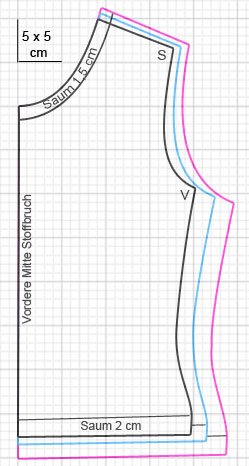
\includegraphics[width=64.54mm]{Front.jpg}
      \caption{Front Pattern}
      \label{fig:Front}
\end{figure}

These are the sample equations for the design
% For single equations
\begin{equation}
 b = h + t\\
\end{equation}

% This is the code for multiple equation
\begin{eqnarray}
%if you want no number to the equation then use \nonumber
a & = & b + c \\
& = & d + e \\
& = & f + g 
\end{eqnarray}
%%%%%%%

%%%%%%%
\subsubsection{Back}

for the back portion all the details are written here

\begin{figure}[ht!]
     \centering
     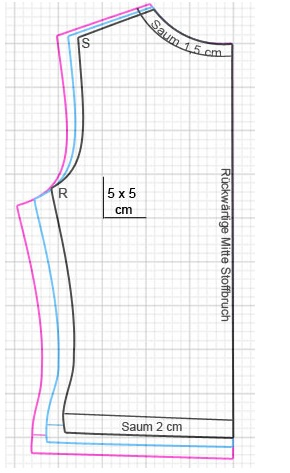
\includegraphics[width=64.54mm]{Back_pattern.jpg}
      \caption{Back Pattern}
      \label{fig:Back}
\end{figure}

These are the equations for back portion
% For single equations
\begin{equation}
 b = h + t\\
\end{equation}


% This is the code for multiple equation
\begin{eqnarray}
%if you want no number to the equation then use \nonumber
a & = & b + c \\
& = & d + e \\
& = & f + g
\end{eqnarray}
%%%%%%%

%%%%%%%
\subsubsection{Sleeve}

for the sleeve portion all the details are written here

\begin{figure}[ht!]
     \centering
     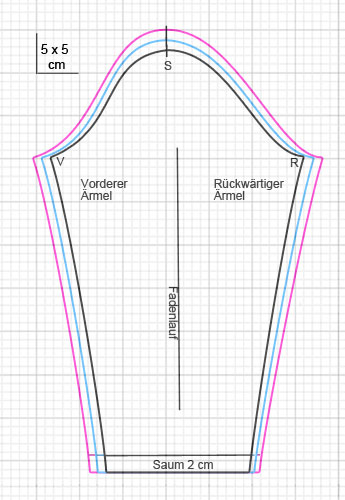
\includegraphics[width=64.54mm]{Sleeve.jpg}
      \caption{Sleeve Pattern}
      \label{fig:Sleeve}
\end{figure}

% For single equations
\begin{equation}
 b = h + t\\
\end{equation}

% This is the code for multiple equation
\begin{eqnarray}
%if you want no number to the equation then use \nonumber
a & = & b + c \\
& = & d + e \\
& = & f + g
\end{eqnarray}
%%%%%%%

%%%%%%
\subsection{Figure Captions}

See figure~\ref{fig:Front} on page~\pageref{fig:Front}.
%%%%%%%

%%%%%%%
\subsection{Table Captions}

See table~\ref{tab:Table 1} for the detailed analysis
%%%%%%%

\end{comment}



\end{document}
